\documentclass[11pt,regno]{amsart}
%\setlength{\hoffset}{-.5in}
\setlength{\voffset}{-.25in}
\usepackage{amssymb,latexsym}
\usepackage{graphicx}
\usepackage{url}		%does nice formatting of URLs
\usepackage{amsfonts,amsmath,amssymb,amsthm}
\usepackage{bm,nicefrac}
\usepackage{siunitx}
\usepackage{derivative}
\usepackage{amsmath,amssymb}
\usepackage{setspace}
\usepackage{csquotes}
\usepackage{caption}
\DeclareRobustCommand{\bbone}{\text{\usefont{U}{bbold}{m}{n}1}}

\DeclareMathOperator{\EX}{\mathbb{E}}% expected value

\textwidth=6.175in
\textheight=9.0in
\headheight=13pt
\calclayout



\newcommand{\R}{{\mathbb R}}
\newcommand{\Q}{{\mathbb Q}}
\newcommand{\C}{{\mathbb C}}
\newcommand{\N}{{\mathbb N}}
\newcommand{\Z}{{\mathbb Z}}

\theoremstyle{plain}
\numberwithin{equation}{section}
\newtheorem{thm}{Theorem}[section]
\newtheorem{theorem}[thm]{Theorem}
\newtheorem{lemma}[thm]{Lemma}
\newtheorem{example}[thm]{Example}
\newtheorem{definition}[thm]{Definition}
\newtheorem{proposition}[thm]{Proposition}

\newcommand{\helv}{%
  \fontfamily{phv}\fontseries{m}\fontsize{9}{11}\selectfont}

\begin{document}
%% replace the values in the next three lines by the correct information
\setcounter{page}{1}

\title{}
\author{}
\thispagestyle{plain}
\begin{center}
    \Large
    \textbf{Assignment 6}
        
    \vspace{0.4cm}
    \large
    \textbf{David Nieves Acarón \& Sam Sharp}
        
    \vspace{0.4cm}
    \textbf{MTH-5324}
    
    \vspace{0.4cm}
    \textbf{Dr. Nezamoddin N. Kachouie}

    \vspace{0.4cm}
    \textbf{Spring 2023}
\end{center}
\email{dnievesacaro2018@my.fit.edu csharp2021@my.fit.edu}
\thanks{}








\maketitle % generates the title of the paper 
\newpage
\doublespacing
\textbf{\section*{Introduction}}
In this report, we are concerned with the modelling of count data for a dataset which covers the salaries of various people across the variables of their gender, work class, education and race. We model two separate datasets, one which contains all the salary data and another which contains only the data of those who make $\$ 50,000$ or more, with the data being altered to portray the count of these individuals for every subclass. In both models, we consider the salary (or the count of salary above the threshold) as the dependent variable and the classifying variables of race, gender, education, and work class as the the independent variables, although the count dataset does not include education. The first model is done using multiple regression, while the second model switches form to a generalized linear model since we are now working with count data. Particularly, we encounter overdispersion of the data which leads us to employ a negative binomial model.

Our essential goal is to ascertain how much someone's race, gender, education, or work class affects their salary. Is there a connection between a higher income and these variables? This problem is important as there is much discussion today about differences in salary outcomes between those of different race and gender. Moreover, this effort could facilitate seeing which occupations and educational attainments could lead to higher incomes as well. 

Modelling done in R provides us the opportunity to quantify just how much these variables might explain incomes, and allow us to see the difference between different combinations. Both multiple regression and negative binomial models are employed.

\textbf{\section*{II. Methods}}


The instructions call for a modelling of the salary based on predictors such as \texttt{age}, \texttt{race}, \texttt{gender}, \texttt{workclass}, \texttt{education}, \texttt{education.num}, and \texttt{hours.per.week} using multiple regression. First, the data is loaded using the standard \texttt{read.csv} function. Next, the data is processed by aggregating all the unique values of gender, age, and race using the \texttt{unique} function. Then, an iteration is made for every unique age, gender, and race for which the number of data points that match that criteria is selected using the \texttt{which} and \texttt{nrow} functions. Finally, this count is then added to a dataframe which is then used by the standard \texttt{lm} function and analyzed with the ols functions provided by the OLSRR library. 


Generalized Linear Modelling is used in statistical analysis by predicting a response $y$, from a linear predictor of the form 
\begin{equation} \tag{1}
X \beta = \beta_0 + X_1 \beta_1 + \dots + \X_k \beta_k 
\end{equation}

As mentioned in the textbook, a generalized linear model involves five main components: some response data in the form of a vector $y = (y_1, \dots , y_n)$, a matrix of predictors $X$, and a vector of coefficients $\beta$, which forms the linear predictor $X\beta$,  a link function $g$, which yields a vector of transformed data in the form, 

\begin{equation} \tag{2}
\hat{y} = g^{-1} (X\beta)
\end{equation} 

  a distribution of data, and finally, some optional parameters to account for variances and overdispersion. Specifically, the Poisson and Negative Binomial models are some of the ones used for count data and as such, are the ones that will be used in this project.

Using the poisson distribution, the regression model is given by the form:

\begin{equation} \tag{3}
y_i \sim \text{Poisson} (e^{\beta_0 + X_1 \beta_1 + \dots + \X_k \beta_k })
\end{equation}

A \texttt{glm.nb} function is used to fit a Negative Binomial Generalized Linear Model. Just like in the previous part, the count is used as the response, with the race, gender, and working class as the predictors. Using the negative binomial model instead of the Poisson model, the effects of overdispersion can be mitigated. Naturally, the model is then of the form:

\begin{equation} \tag{4}
y_i \sim \text{Negative Binomial} (e^{\beta_0 + X_1 \beta_1 + \dots + \X_k \beta_k })
\end{equation} 

When we deal with data that has a response variable of integer type, using a linear regression may violate the normality assumption. Thus, we employ a generalized linear model with a Negative Binomial distribution, of which the Poisson Distribution is a special case \cite{book}.

Finally, we note that for regression of categorical variables, the summary outputs in R lack one category for each variable, which we will denote as the reference variable. These reference variables are absorbed into the intercept and is used as a a baseline to compare the rest of the categories. Every categorical variable then thus has $k -1$ dummy variables to ensure safety from perfect multicollinearity (page 136 of \cite{book}).


\textbf{\section*{Results}}
Concerning the multiple regression model modeling the salaries, multiple predictors and their categories were deemed statistically significant, these can be seen in Table 2. Our reference intercept was chosen from the dummy variable combination of a female American Indian clerical worker whose education stopped at the tenth grade level. This was also deemed significant with an estimate coefficient of $-24.624$. 

Regarding the negative binomial model, Table 1 shows the statistically significant variables with their associated intercepts. Similarly, the reference intercept was the case of a female Native American clerical worker, which was also statistically significant with an estimate of $2.27$. The multiple regression model had an adjusted $R^2$ value of $0.1761$. Figure 1 displays some visualization plots for the count data. The difficulty of visualizing this data should not be understated, as the high number of points, the high dimensionality, and the overabundance of the majority classes can complicate such as visualization.

\begin{figure}[h!]  
\caption*{\textit{Table 1:} Statistically significant variables and their coefficient estimates for the negative binomial model.}
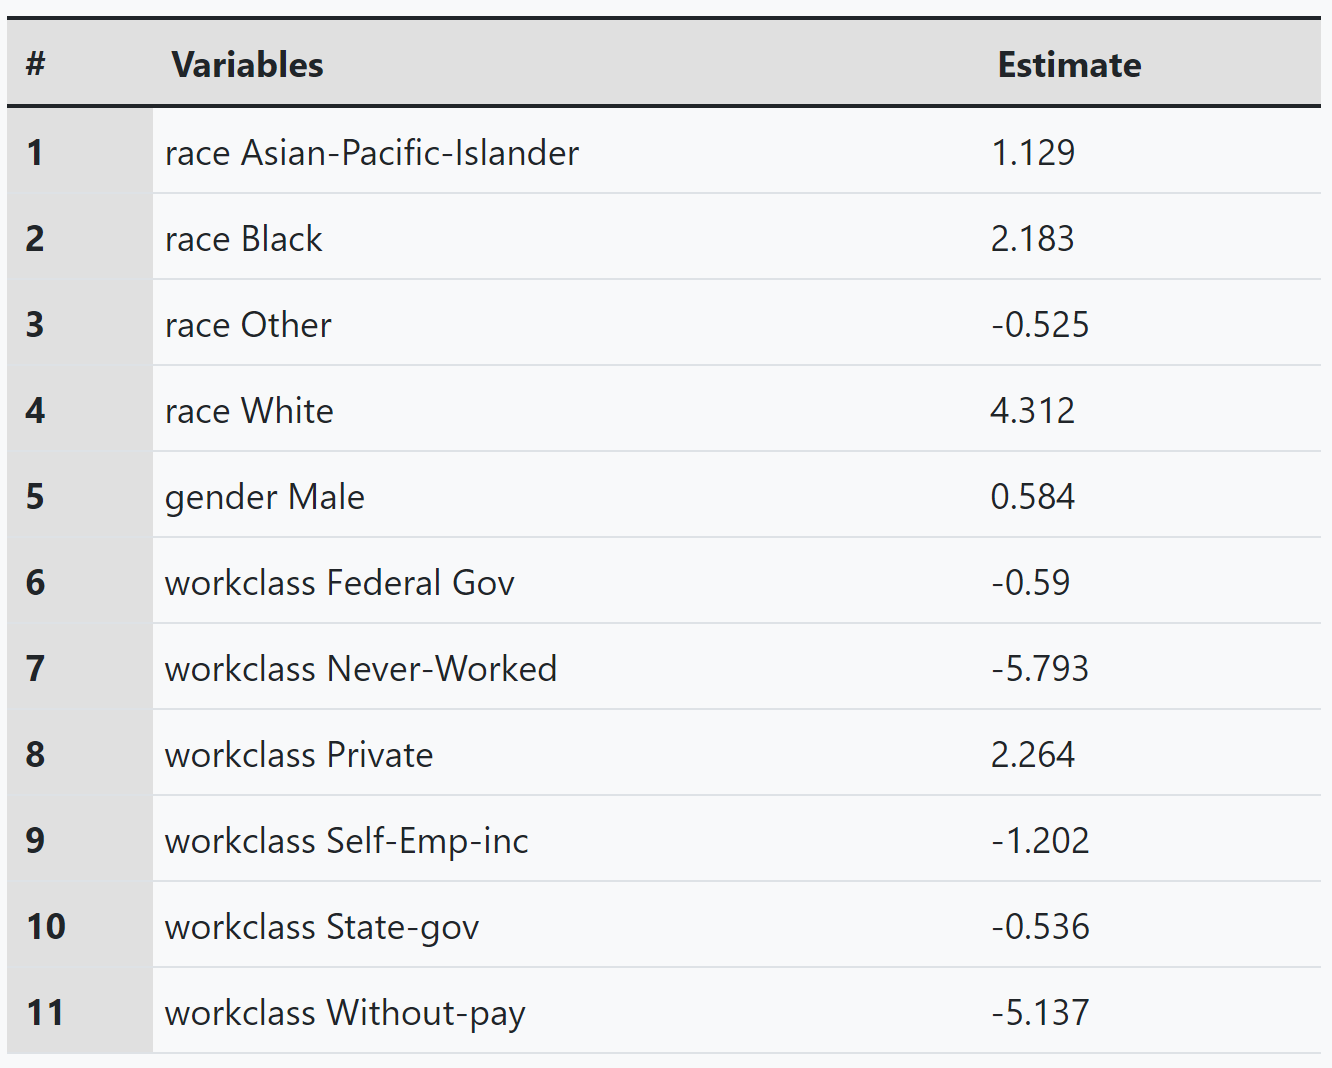
\includegraphics[scale = 0.4]{assignment6/tablesest2.png} 
\end{figure}

\begin{figure}[h!]  
\caption*{\textit{Table 2:} Statistically significant variables and their coefficient estimates for the multiple regression model.}
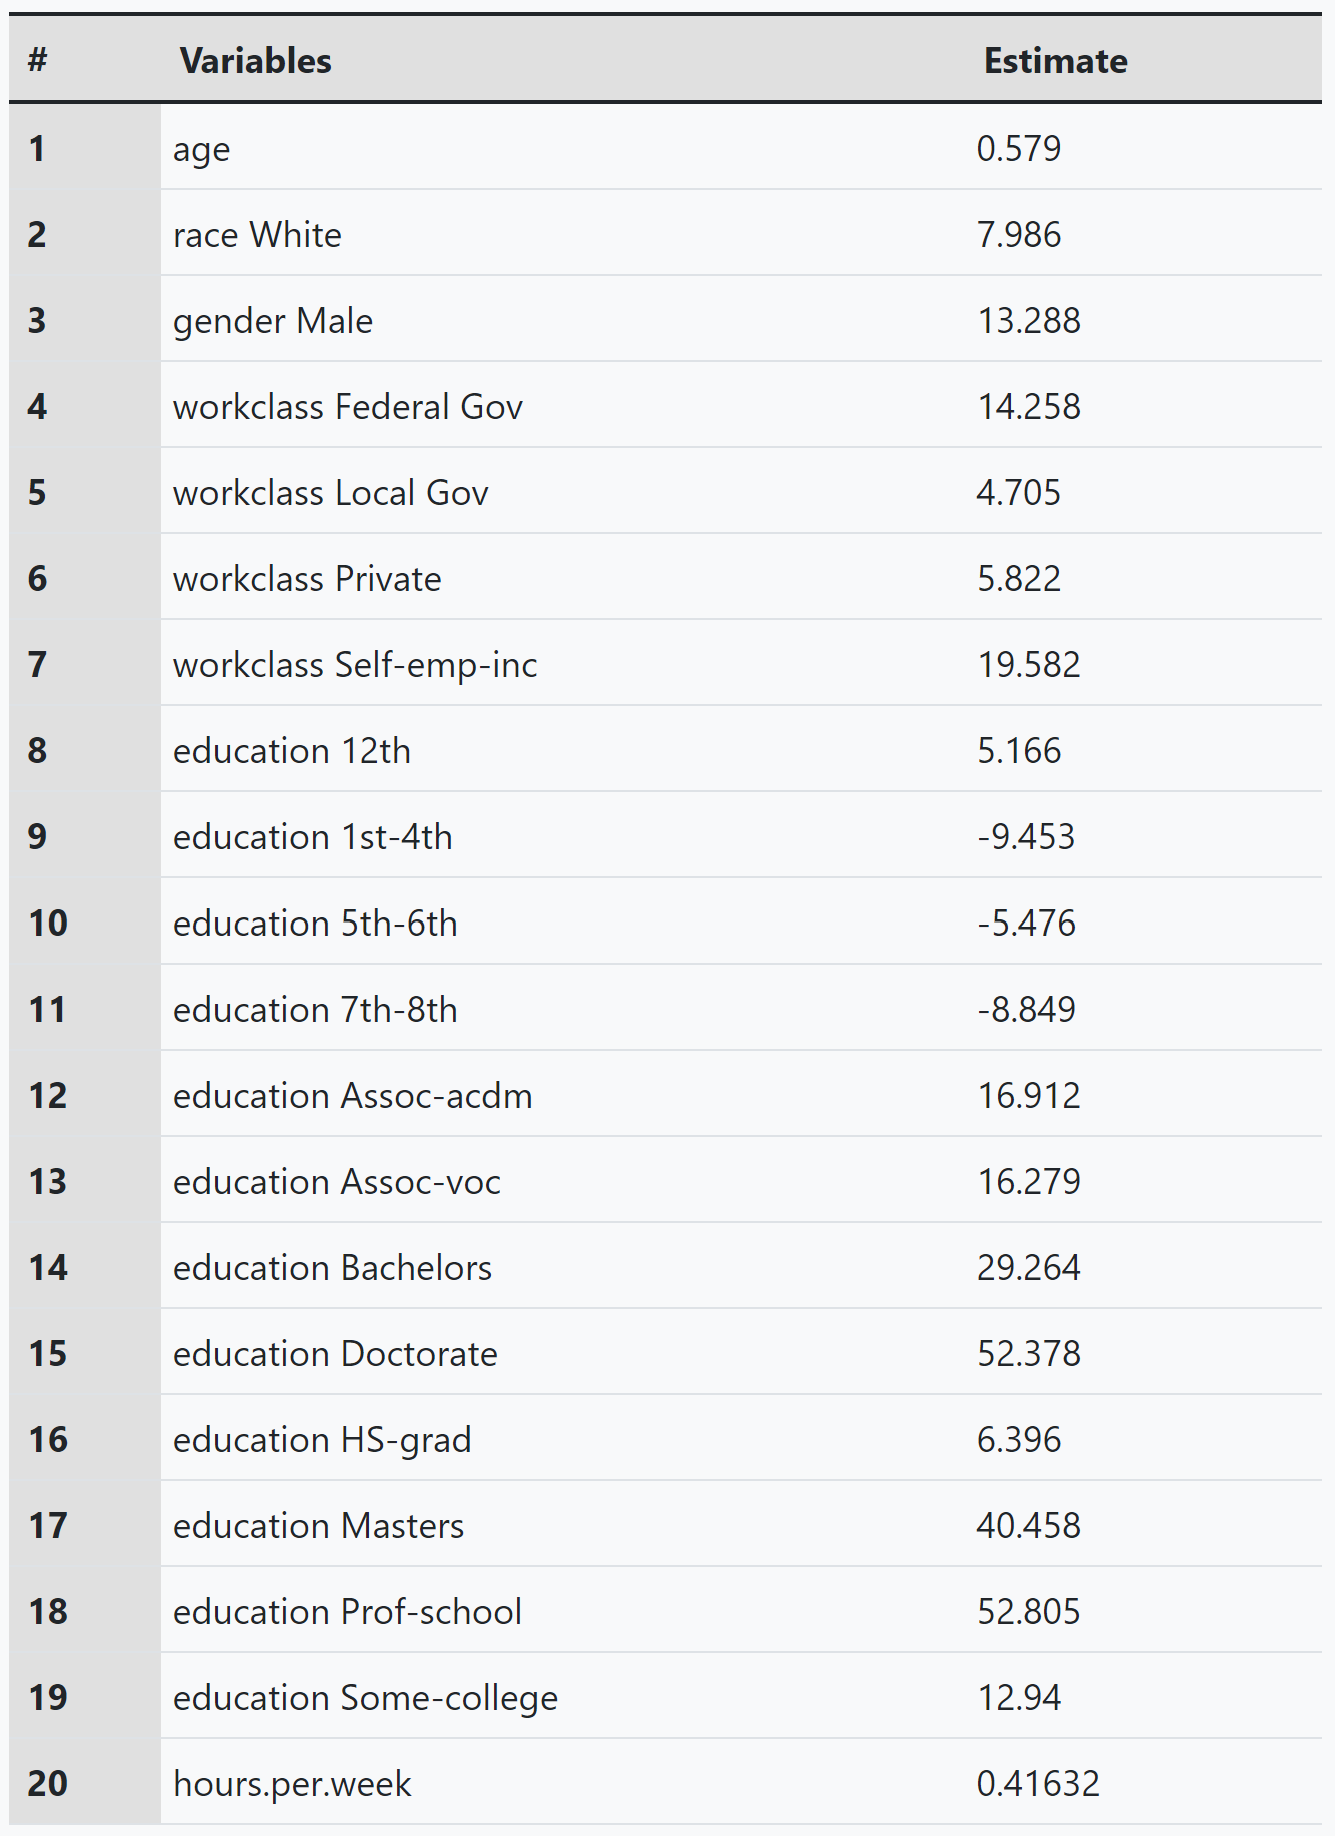
\includegraphics[scale = 0.6]{assignment6/tablesEstimates.png} 
\end{figure}


\begin{figure}
\centering
\centerline{ \mbox{
\subfigure{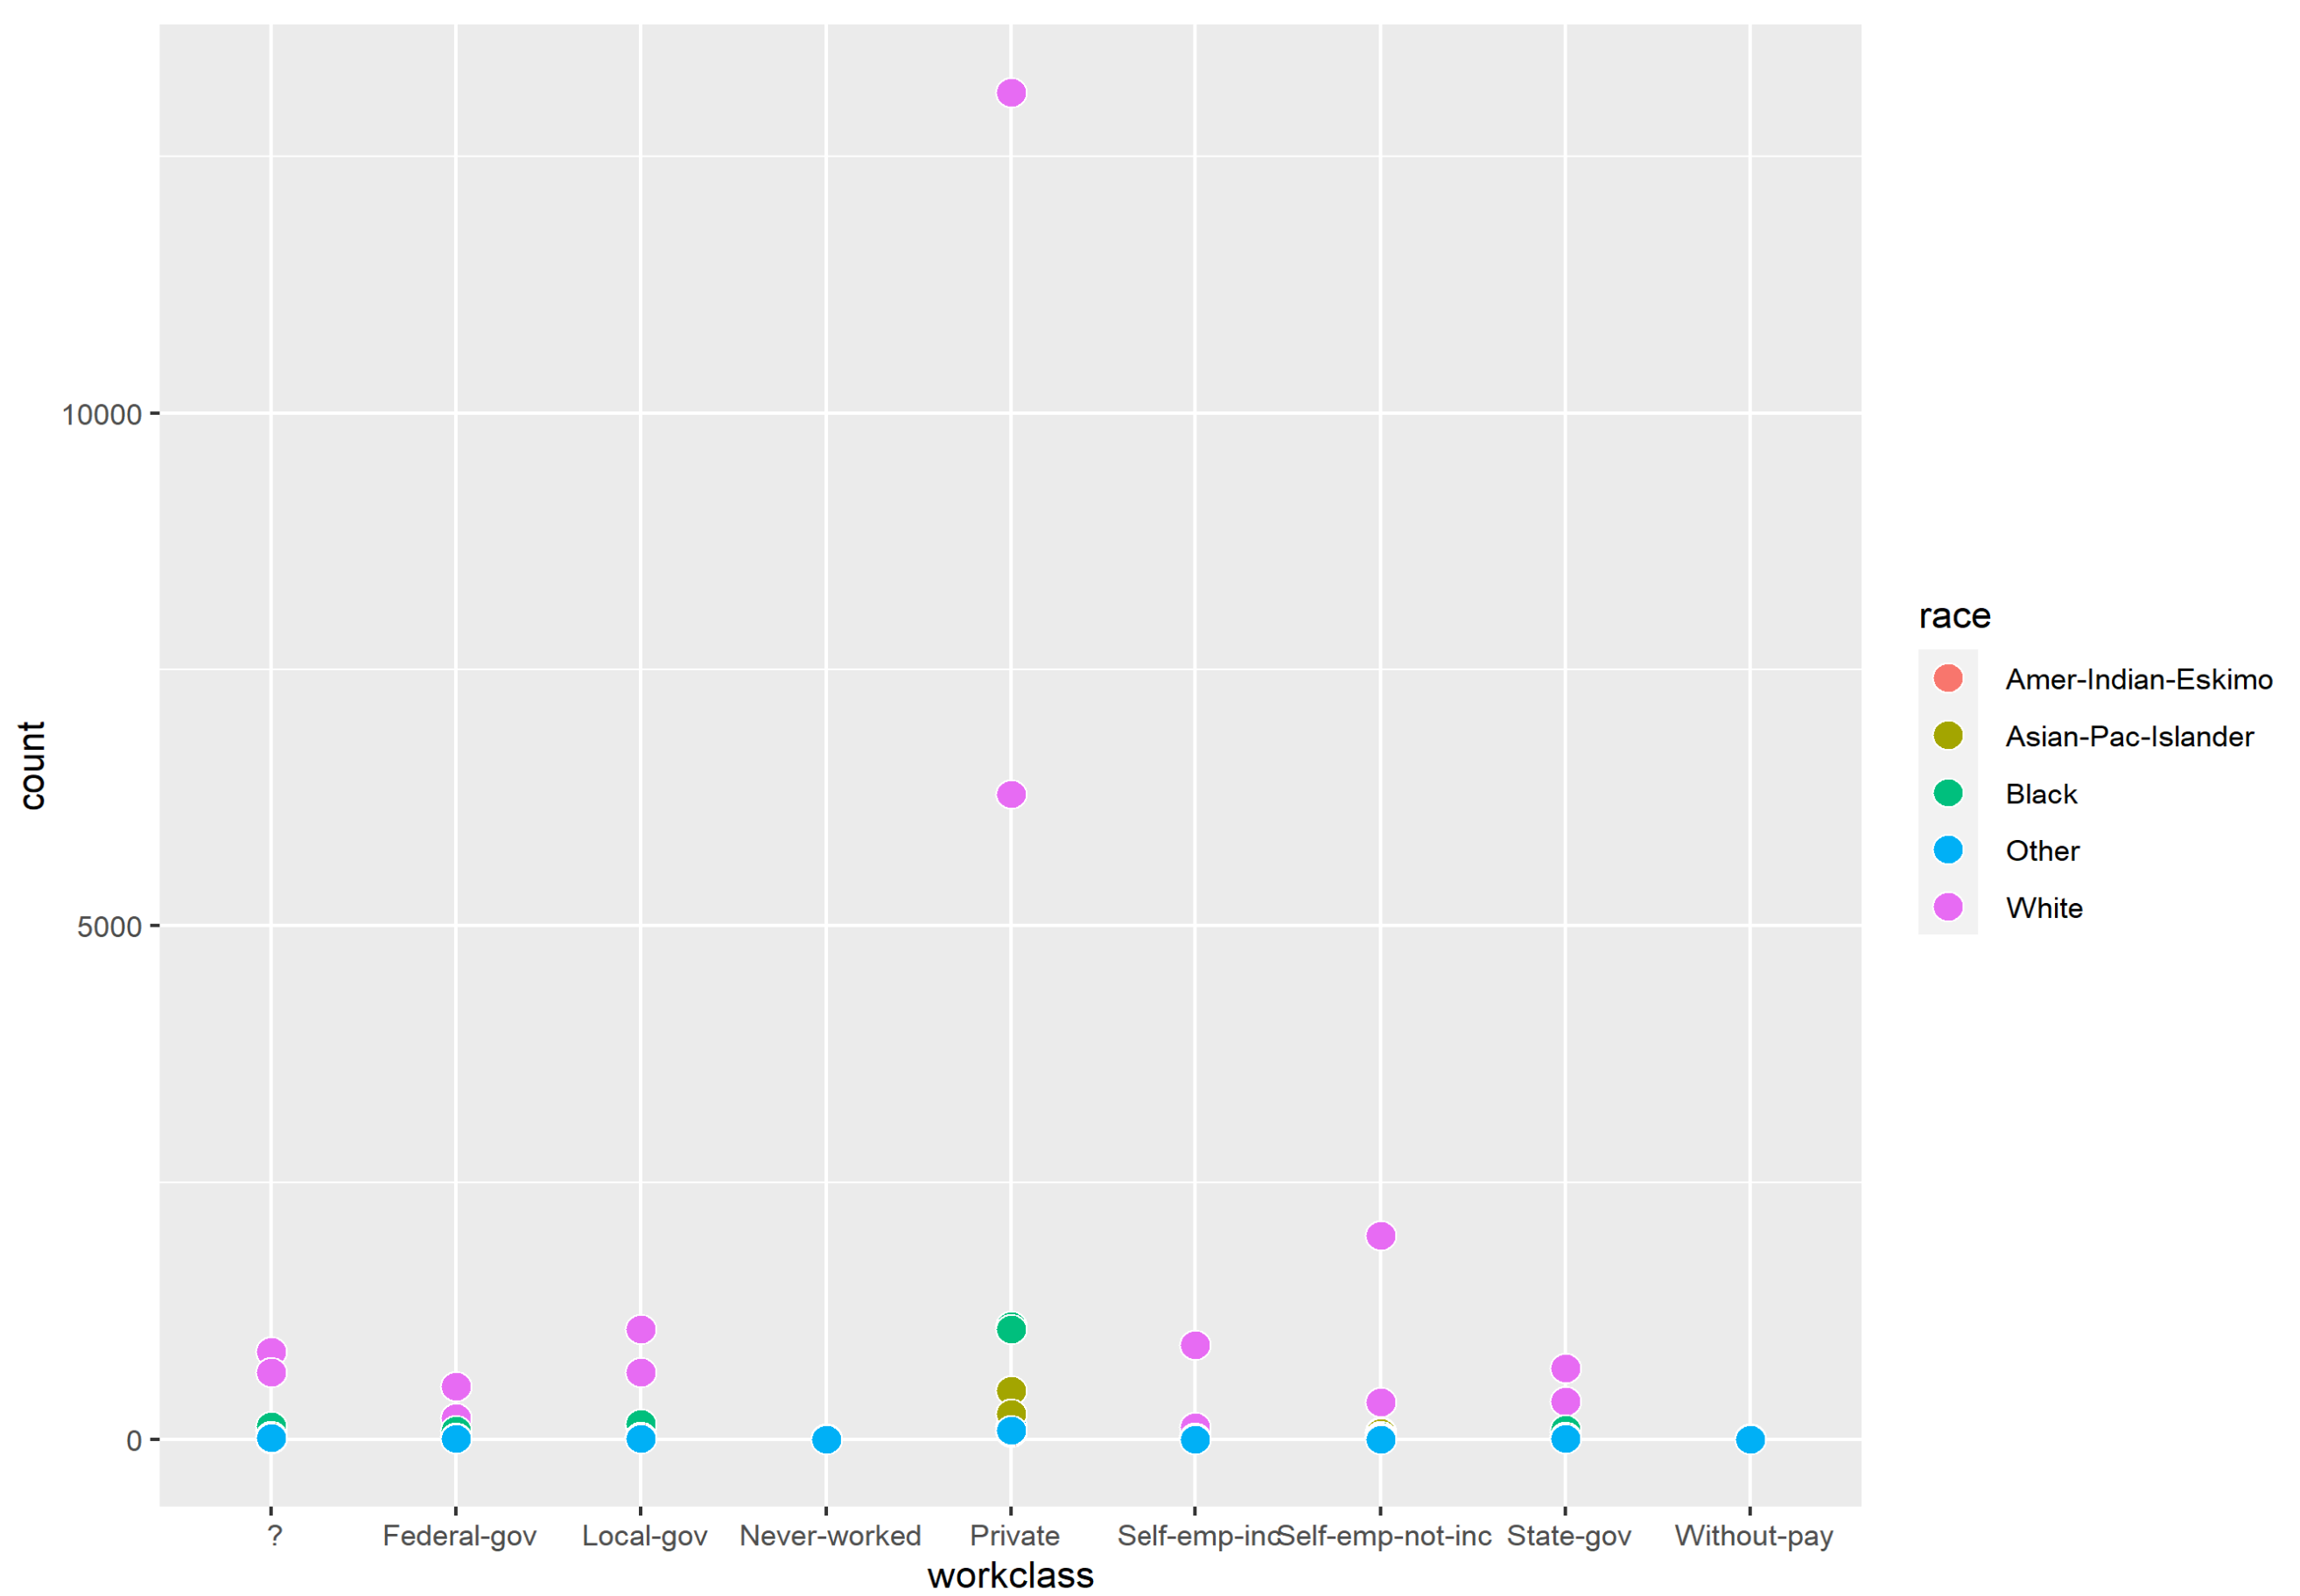
\includegraphics[width=3in]{count-class.png}}\quad
\subfigure{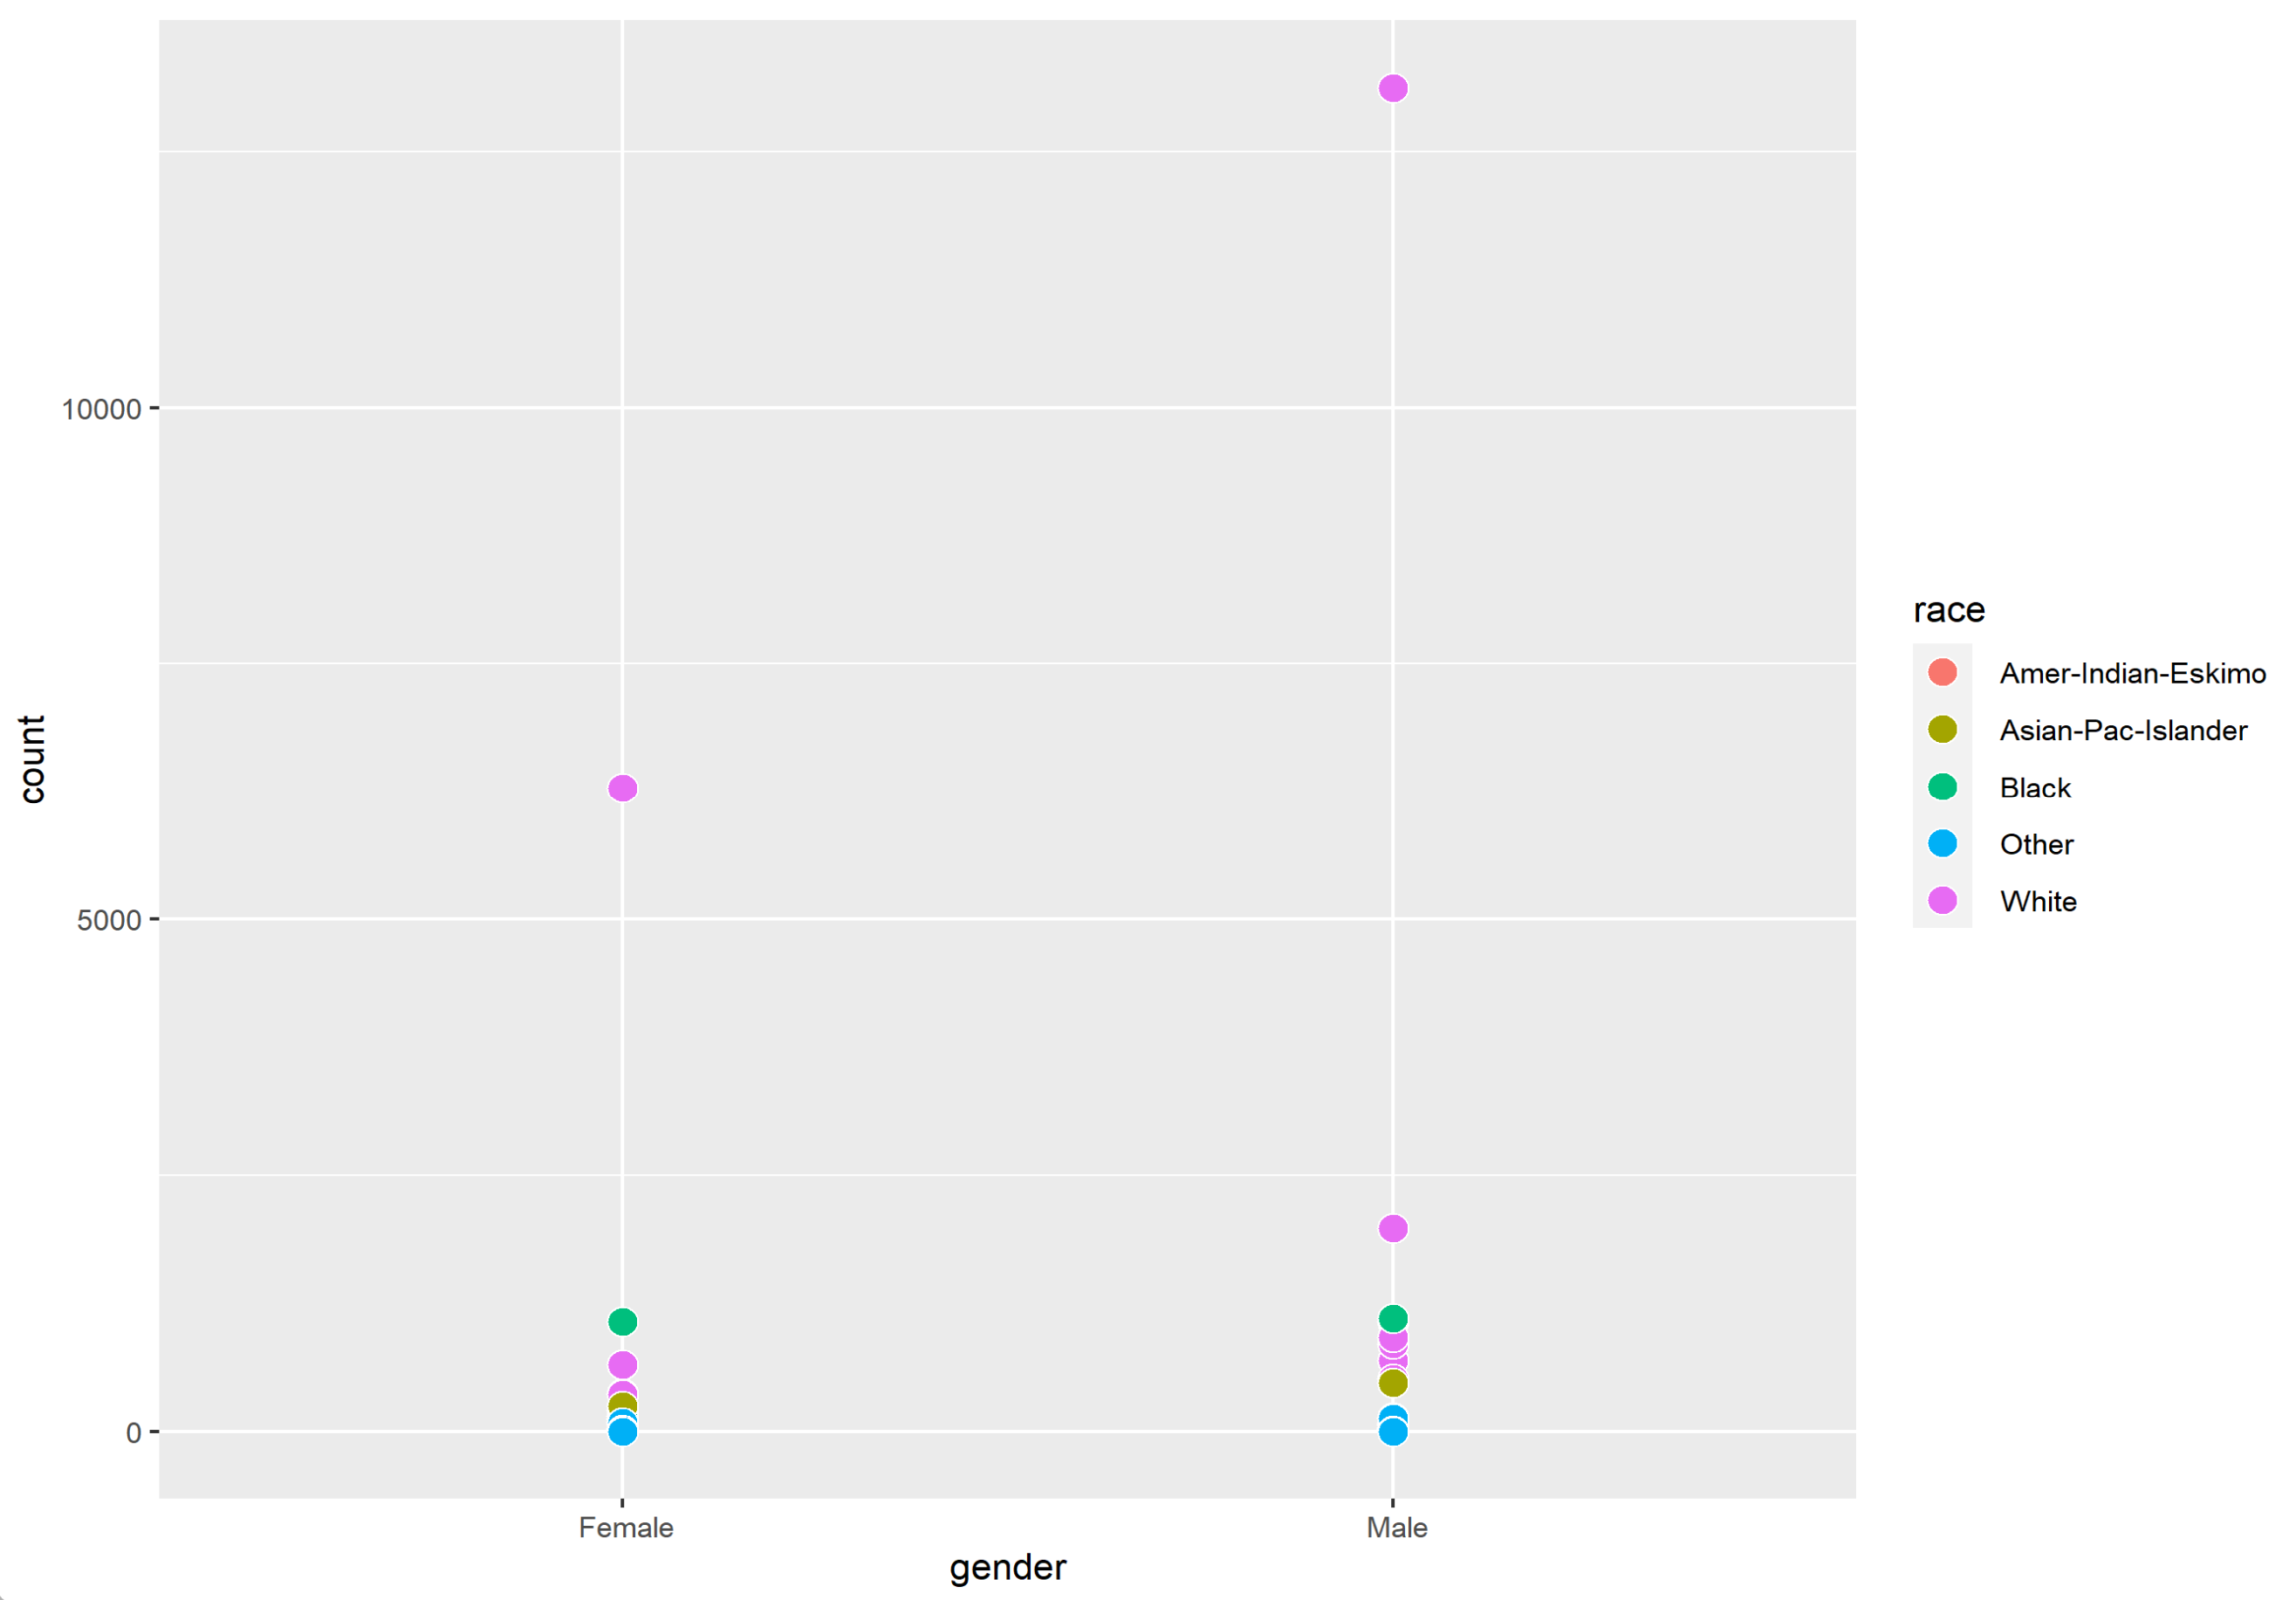
\includegraphics[width=3in]{count-gender.png}} }}
\caption{Figures showing visualizations of count data using different variables as the x axis. }
\end{figure}

\ 

\ 


\ 




 


%%%%%%%%\end{table}


% \begin{table}[]
% \caption*{\textit{Table 3:} $\theta$ and Standard error of the Negative Binomial model..}
% \begin{tabular}{|l|l|}
% \hline
% $\theta$    & 4.804 \\ \hline
% Std. Err & 0.986 \\ \hline
% \end{tabular}
% \end{table}




  
\textbf{\section*{Discussion and Conclusion}}
To begin, we find  many statistically significant predictors for an individual's salary using the multiple regression model. Among the most prevalent by far those with the highest estimates, are the levels of education the individual has achieved. With the reference with respect to education being that of completion of tenth grade clerk, we see accordingly lower education levels having negative responses while higher education levels have increasingly higher responses. Interestingly, we see the estimates for those with Doctorates and Professional school backgrounds having quite similar responses. Among significant work class predictors, all in Table 1 show positive responses in comparison to the reference of an  administrative clerk. A value of white for race seems to lead to higher salaries in comparison to those of Native American ancestry, while males seem to have higher salaries than females. We additionally see a positive correlation between an increasing age and salary. The adjusted $R^2$ was a mere $0.1761$, which leads us to believe there are many other significant factors which might effect an individual's salary, such as nationality, major in college, and ancestral wealth.

Regarding the negative binomial model, we see some similar results for predicting whether an individual will have a salary of greater than 50,000 dollars. With respect to race and the Native American reference variable, we see a higher propensity for Black, Asian-Pacific-Islander, and White individuals having salaries over fifty thousand, while "other" has a lesser propensity (it is not quite known what ethnicity other denotes). Again, with respect to gender, we see males having a positive response in comparison to the reference variable female. Among working classes, variables against the reference variable of administrative clerk positions with worse count responses include Federal Government, State Government, No work, Work without pay, and Self employed positions. The only positive response with respect the administrative clerk positions was private industry. We infer from the results of both models that then administrative clerk positions have a high likelihood of putting an individual in the greater than fifty thousand bracket, without much of an upward possible climb in salary as you would see from private industry or lucrative self employment roles. This can be seen in Figure 1 which does show a large jump in count for individuals working in private industry, as well as a gap between incomes between men and women.



For future efforts, other distributions could be employed to model this count data. If the data were to include many zeroes, a zero-inflated model could be used. Furthermore, there is potential in adding other interesting variables to this data such as religious affiliation, location in nation, or general health.





















\newpage

\section*{References}
\begingroup
\renewcommand{\section}[2]{}%
\begin{thebibliography}{9}


\bibitem{boes}
Kachouie, Nezzamodin N. (2023): 
Class Notes 



\bibitem{cinco}
A. Colin Cameron and Pravin K. Trivedi (2013), Regression Analysis of Count Data, 2nd edition,
Econometric Society Monograph No.53, Cambridge University Press, 1998 (566 pages.)

\bibitem{book}
Gelman A, Hill J., and Vehtari A. (2020)  Regression and Other Stories, Cambridge University Press

\end{thebibliography}
\endgroup

\

\

\

\end{document}